\documentclass[11pt,a4paper]{article}

% ============================================
% PACKAGES
% ============================================
\usepackage[utf8]{inputenc}
\usepackage[T1]{fontenc}
\usepackage{amsmath,amssymb,amsthm}
\usepackage{mathtools}
\usepackage{physics}
\usepackage{geometry}
\usepackage{graphicx}
\usepackage{float}
\usepackage{booktabs}
\usepackage{enumitem}
\usepackage{hyperref}
\usepackage{cleveref}
\usepackage{tikz}
\usepackage{pgfplots}
\usepackage{xcolor}

% TikZ libraries
\usetikzlibrary{
    arrows.meta,
    calc,
    decorations.markings,
    decorations.pathmorphing,
    patterns,
    shapes.geometric,
    positioning,
    3d,
    backgrounds,
    shadings,
    fadings
}

\pgfplotsset{compat=1.18}

% ============================================
% PAGE GEOMETRY
% ============================================
\geometry{
    left=2.5cm,
    right=2.5cm,
    top=2.5cm,
    bottom=2.5cm
}

% ============================================
% CUSTOM COLORS
% ============================================
\definecolor{substrate}{RGB}{230,240,250}
\definecolor{curvature}{RGB}{70,130,180}
\definecolor{matter}{RGB}{180,60,60}
\definecolor{relaxation}{RGB}{60,140,60}
\definecolor{stable}{RGB}{140,80,160}
\definecolor{energy}{RGB}{200,120,50}

% ============================================
% THEOREM ENVIRONMENTS
% ============================================
\theoremstyle{definition}
\newtheorem{definition}{Definition}[section]
\newtheorem{constraint}{Constraint}[section]

\theoremstyle{plain}
\newtheorem{proposition}{Proposition}[section]

\theoremstyle{remark}
\newtheorem{remark}{Remark}[section]

% ============================================
% CUSTOM COMMANDS
% ============================================
\newcommand{\Egeom}{E_{\text{geom}}}
\newcommand{\meff}{m_{\text{eff}}}
\newcommand{\lc}{\ell_c}

% ============================================
% TITLE AND AUTHORS
% ============================================
\title{\textbf{On the Geometric Origin of Matter\\in Emergent Gravity Frameworks}\\[0.5em]\large BP3.5}
\author{
Lee Smart \\
Vibrational Field Dynamics Institute \\
Email: contact@vibrationalfielddynamics.org \\
X (Twitter): @vfd\_org
}
\date{December 4 2025}

% ============================================
% DOCUMENT
% ============================================
\begin{document}

\maketitle

% ============================================
% ABSTRACT
% ============================================
\begin{abstract}
\noindent If gravity emerges from geometric relaxation dynamics rather than constituting a fundamental force, then the ontological status of matter requires re-examination. This paper argues that within a consistent emergent gravity framework, matter cannot be ontologically independent of the geometric substrate from which gravity itself arises. We define matter as geometric configurations that resist relaxation under the same dynamics that produce emergent gravitational behaviour. This definition is a necessary consequence of ontological consistency rather than an auxiliary hypothesis. Mass, inertia, and gravitational coupling follow naturally from this geometric characterisation, and the transition to discrete behaviour emerges from stabilisation constraints. Full derivation of quantum dynamics is deferred to subsequent work.
\end{abstract}

\vspace{1em}
\hrule
\vspace{1em}

\tableofcontents

\newpage

% ============================================
% SECTION 1: INTRODUCTION
% ============================================
\section{Introduction}
\label{sec:introduction}

Previous work (BP3) established that gravitational phenomena can be understood as emergent properties of a geometric substrate undergoing curvature relaxation. In that framework, gravity is not a fundamental force mediated by exchange particles or imposed as a primitive interaction, but rather the macroscopic manifestation of an underlying geometric dynamics seeking configurations of minimal curvature distortion. The Einstein field equations emerge as an effective description in regimes where the substrate exhibits sufficient coherence, as established in BP3.

\textbf{Continuity with BP3.} This paper assumes the results of BP3 without rederivation. The emergence of gravity from geometric relaxation is taken as established, and we do not reproduce those arguments here. Gravity enters only as a foundational constraint---an axiom from which further consequences follow. The present work extends BP3 by addressing a question it necessarily raises but does not answer: \emph{if gravity is geometric in origin, what is matter?}

The standard approach treats matter and geometry as ontologically distinct categories---matter as a collection of fundamental particles obeying quantum field dynamics, geometry as a background or dynamical arena that matter inhabits and curves. However, if gravity is not fundamental but emergent from geometry, this dual ontology becomes problematic. Matter that curves spacetime must interact with the same geometric substrate from which gravity emerges. Whether matter can remain ontologically independent of this substrate is not merely philosophical but has direct implications for the internal consistency of the framework.

We argue that ontological consistency demands matter be understood as a particular class of geometric configurations---specifically, those that resist the relaxation dynamics from which gravity emerges. This is not a speculative identification but a logical requirement. The central claim is minimal: \textbf{matter is stabilised geometry}.

\medskip
\noindent\textit{Takeaway:} The question of matter's ontological status is forced upon us by emergent gravity; this paper provides a minimal, consistent answer.

% ============================================
% SECTION 2: EMERGENT GRAVITY AS CONSTRAINT
% ============================================
\section{Emergent Gravity as a Foundational Constraint}
\label{sec:emergent-gravity}

We adopt as foundational constraints the following results established in BP3:

\begin{constraint}[Single Substrate]
\label{con:substrate}
There exists a single geometric substrate characterised by a metric structure $g$ and associated curvature quantities. All physical phenomena derive from configurations of this substrate.
\end{constraint}

\begin{constraint}[Scale-Dependent Coherence]
\label{con:coherence}
The substrate exhibits coherent behaviour above a characteristic length scale $\lc$. Below this scale, the effective description in terms of smooth differential geometry may require modification.
\end{constraint}

\begin{constraint}[Relaxation Dynamics]
\label{con:relaxation}
The substrate evolves according to dynamics that reduce curvature distortion. This relaxation process, when viewed at macroscopic scales, produces the phenomenology described by general relativity.
\end{constraint}

These constraints are axioms from which consequences are derived, not hypotheses under test. The curvature content of the substrate is captured by a functional $R[g]$ measuring departure from flatness. The substrate evolves to reduce this functional, subject to boundary conditions and topological constraints.

Symbolically, the relaxation dynamics take the form:
\begin{equation}
\label{eq:relaxation}
\partial_t g = -\mathcal{F}\left[\frac{\delta R}{\delta g}\right]
\end{equation}
Here $t$ is interpreted as a relaxation (gradient-flow) parameter rather than physical time. The functional $R[g]$ denotes a scalar curvature measure (e.g., an integrated curvature invariant), and $\mathcal{F}$ represents a local operator mapping symmetric tensor variations to symmetric tensor variations. Gauge and diffeomorphism issues are not fixed at this stage, as only the existence of a relaxation direction is required for the argument.

The essential point is that this dynamics defines a preferred direction of evolution: toward configurations of reduced curvature content. Any configuration that persists against this tendency requires explanation.

\begin{figure}[H]
\centering
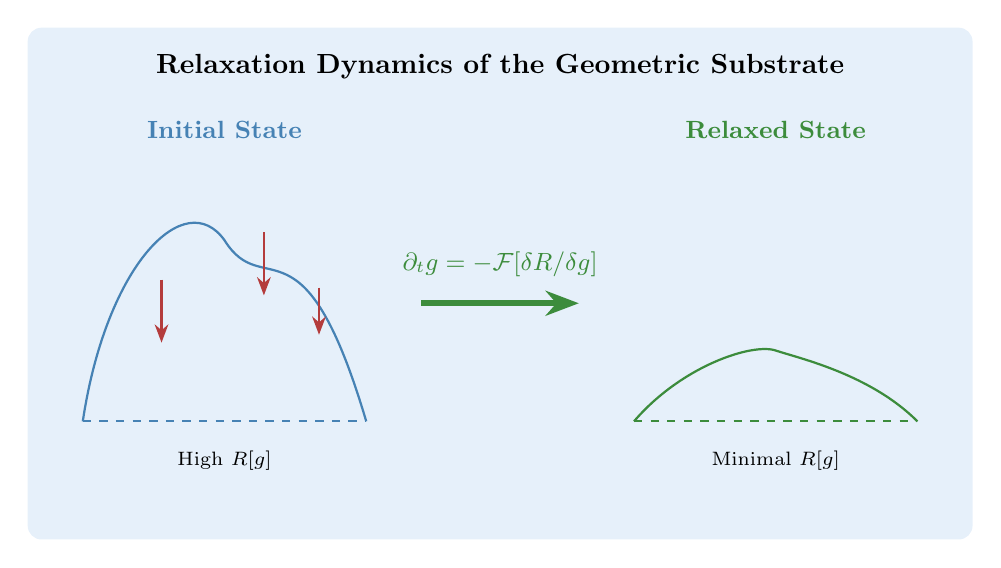
\begin{tikzpicture}[scale=1.0]
    % Background
    \fill[substrate, rounded corners=5pt] (-6,-3) rectangle (6,3.5);

    % Title
    \node[font=\bfseries] at (0,3) {Relaxation Dynamics of the Geometric Substrate};

    % Left panel: High curvature (initial)
    \begin{scope}[shift={(-3.5,0)}]
        \node[font=\small\bfseries, curvature] at (0,2.2) {Initial State};
        \draw[thick, curvature] (-1.8,-1.5)
            .. controls (-1.5,0.5) and (-0.5,1.5) .. (0,0.8)
            .. controls (0.5,0) and (1,1.2) .. (1.8,-1.5);
        \draw[thick, curvature, dashed] (-1.8,-1.5) -- (1.8,-1.5);

        % Curvature indicators
        \draw[-{Stealth}, thick, matter] (-0.8,0.3) -- (-0.8,-0.5);
        \draw[-{Stealth}, thick, matter] (0.5,0.9) -- (0.5,0.1);
        \draw[-{Stealth}, thick, matter] (1.2,0.2) -- (1.2,-0.4);

        \node[font=\scriptsize] at (0,-2) {High $R[g]$};
    \end{scope}

    % Arrow
    \draw[-{Stealth}, very thick, relaxation, line width=2pt] (-1,0) -- (1,0);
    \node[font=\small, relaxation] at (0,0.5) {$\partial_t g = -\mathcal{F}[\delta R/\delta g]$};

    % Right panel: Low curvature (relaxed)
    \begin{scope}[shift={(3.5,0)}]
        \node[font=\small\bfseries, relaxation] at (0,2.2) {Relaxed State};
        \draw[thick, relaxation] (-1.8,-1.5)
            .. controls (-1.2,-0.8) and (-0.3,-0.5) .. (0,-0.6)
            .. controls (0.3,-0.7) and (1.2,-0.9) .. (1.8,-1.5);
        \draw[thick, relaxation, dashed] (-1.8,-1.5) -- (1.8,-1.5);

        \node[font=\scriptsize] at (0,-2) {Minimal $R[g]$};
    \end{scope}
\end{tikzpicture}
\caption{Curvature relaxation. The substrate evolves from high-curvature configurations (left) toward minimal-curvature configurations (right) under the dynamics of \cref{eq:relaxation}. Arrows indicate local curvature reduction. (Note: All figures in this paper are schematic illustrations of geometric concepts; they do not depict physical particles or observable entities.)}
\label{fig:relaxation}
\end{figure}

\medskip
\noindent\textit{Takeaway:} Gravity is not rederived here; it enters as an axiomatic constraint that shapes all subsequent reasoning about matter.

% ============================================
% SECTION 3: INCONSISTENCY
% ============================================
\section{Inconsistency of Independent Matter Ontologies}
\label{sec:inconsistency}

Consider the proposition that matter consists of entities ontologically independent of the geometric substrate---entities possessing properties (mass, charge, spin) as primitive attributes attached to point-like or field-like objects inhabiting the substrate.

This proposition encounters a fundamental difficulty. Independent matter must couple to geometry to produce gravitational effects. In standard general relativity, the stress-energy tensor encodes this coupling. But if gravity is emergent from substrate relaxation, how does ontologically independent matter participate in the relaxation dynamics?

Two possibilities arise:

\textbf{Possibility A:} Independent matter does not participate in substrate dynamics but produces curvature through a separate mechanism.

This creates a dual dynamics problem. The substrate would evolve via intrinsic relaxation while being curved by matter through an unrelated process. No natural principle ensures compatibility between these influences. The unification achieved by emergent gravity would be broken.

\textbf{Possibility B:} Independent matter participates in substrate dynamics as an external forcing term.

This raises the question of how ontologically distinct entities can influence geometric degrees of freedom. The substrate is the fundamental arena by hypothesis; entities independent of it lack a natural coupling mechanism. Any ad hoc coupling represents an additional postulate.

Both possibilities introduce complications the emergent gravity framework was designed to avoid. The logical path of least assumption is to deny the initial proposition: \emph{matter is not ontologically independent of the geometric substrate}.

This argument concerns ontological foundations, not empirical adequacy. Theories treating matter and geometry separately may be entirely adequate as effective descriptions. But if one commits to a single geometric substrate as the ground of all physical phenomena, matter must be accommodated within that substrate.

\begin{figure}[H]
\centering
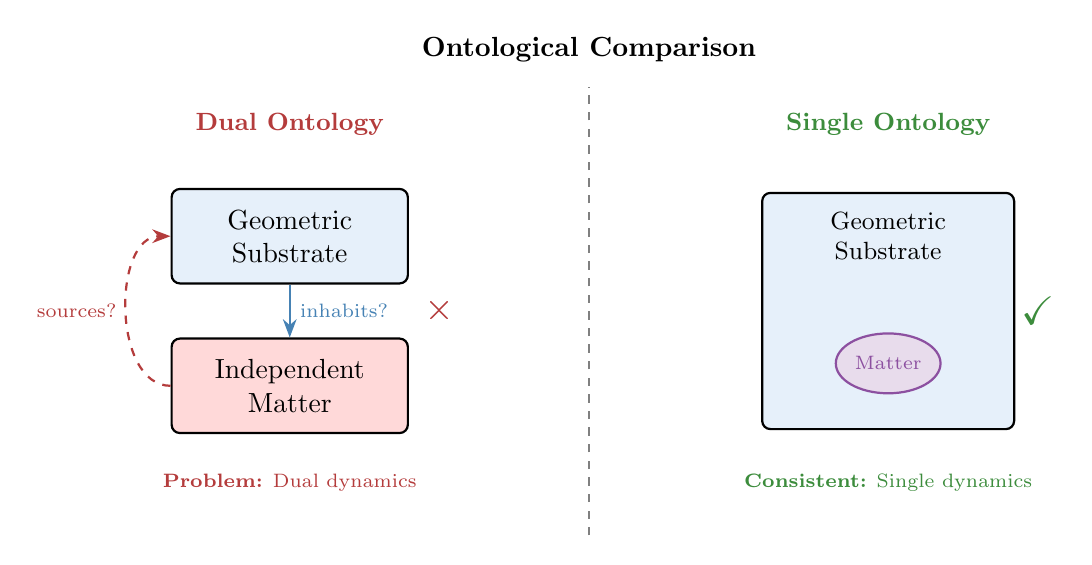
\begin{tikzpicture}[
    box/.style={draw, thick, rounded corners=3pt, minimum width=3cm, minimum height=1.2cm, align=center},
    arrow/.style={-{Stealth}, thick},
    scale=0.95
]
    % Title
    \node[font=\bfseries] at (0,4.5) {Ontological Comparison};

    % Left side: Dual Ontology (Inconsistent)
    \begin{scope}[shift={(-4,0)}]
        \node[font=\small\bfseries, matter] at (0,3.5) {Dual Ontology};

        \node[box, fill=substrate] (geo1) at (0,2) {Geometric\\Substrate};
        \node[box, fill=red!15] (mat1) at (0,0) {Independent\\Matter};

        \draw[arrow, curvature] (geo1.south) -- (mat1.north)
            node[midway, right, font=\scriptsize] {inhabits?};
        \draw[arrow, matter, dashed] (mat1.west) to[out=180,in=180]
            node[midway, left, font=\scriptsize] {sources?} (geo1.west);

        \node[font=\scriptsize, matter] at (0,-1.3) {\textbf{Problem:} Dual dynamics};

        % X mark
        \node[font=\Large, matter] at (2,1) {\texttimes};
    \end{scope}

    % Right side: Single Ontology (Consistent)
    \begin{scope}[shift={(4,0)}]
        \node[font=\small\bfseries, relaxation] at (0,3.5) {Single Ontology};

        % Box for geometric substrate - taller to fit matter inside
        \node[box, fill=substrate, minimum height=3cm, minimum width=3.2cm] (geo2) at (0,1) {};

        % Text at top of box
        \node[font=\small, align=center] at (0,2) {Geometric\\Substrate};

        % Matter ellipse in lower portion of box
        \draw[thick, stable, fill=stable!20] (0,0.3) ellipse (0.7 and 0.4);
        \node[font=\scriptsize, stable] at (0,0.3) {Matter};

        \node[font=\scriptsize, relaxation] at (0,-1.3) {\textbf{Consistent:} Single dynamics};

        % Check mark
        \node[font=\Large, relaxation] at (2,1) {\checkmark};
    \end{scope}

    % Dividing line
    \draw[thick, dashed, gray] (0,-2) -- (0,4);
\end{tikzpicture}
\caption{Ontological comparison. Left: Dual ontology creates unresolved coupling questions. Right: Single ontology maintains consistency with emergent gravity.}
\label{fig:ontology}
\end{figure}

\medskip
\noindent\textit{Takeaway:} Ontological consistency forces matter to be part of the geometric substrate, not independent of it.

% ============================================
% SECTION 4: MATTER AS STABILISED GEOMETRY
% ============================================
\section{Definition: Matter as Stabilised Geometry}
\label{sec:definition}

We propose the following definition:

\begin{definition}[Matter]
\label{def:matter}
\textbf{Matter} consists of geometric configurations of the substrate that resist relaxation under the dynamics from which gravity emerges.
\end{definition}

This definition has three components: (i) what constitutes a configuration, (ii) what constitutes resistance to relaxation, and (iii) what mechanisms enable such resistance.

\subsection{Geometric Configurations}
\label{subsec:configurations}

A configuration $\gamma$ is a specification of the metric $g$ and any additional geometric structures (such as torsion $T$ or non-metricity $Q$) over a region of the substrate. Configurations may be localised, exhibiting significant deviation from background geometry only within a bounded region, or extended over larger scales.

\subsection{Resistance to Relaxation}
\label{subsec:resistance}

The relaxation dynamics drive the substrate toward configurations minimising the curvature functional $R[g]$. A configuration resists relaxation if it does not evolve toward the global minimum---either because it occupies a local minimum or because evolution toward lower curvature is obstructed.

Let $\Egeom[\gamma]$ denote the geometric energy functional associated with configuration $\gamma$:
\begin{equation}
\label{eq:energy-functional}
\Egeom[\gamma] = \int_{\Omega} \mathcal{L}(R, T, \nabla R, \ldots) \, d\mu_g
\end{equation}
where $\Omega$ is the support of the configuration and $\mathcal{L}$ is a Lagrangian density constructed from geometric invariants. For the present argument, the curvature functional $R[g]$ may be regarded as the relevant geometric energy $\Egeom[g]$, up to constants and boundary terms.

A configuration is \emph{stabilised} if it satisfies:
\begin{equation}
\label{eq:stability-first}
\delta \Egeom = 0
\end{equation}
and
\begin{equation}
\label{eq:stability-second}
\delta^2 \Egeom > 0
\end{equation}

The first condition asserts that the configuration is a critical point. The second asserts it is a local minimum, so small perturbations increase energy and are disfavoured by relaxation. In a gradient-descent relaxation regime, such local minima are dynamically stable (up to diffeomorphism gauge freedom).

\subsection{Mechanisms of Stabilisation}
\label{subsec:mechanisms}

Three mechanisms can produce stabilisation:

\textbf{Curvature Trapping.} If the energy functional has multiple local minima separated by barriers, a configuration in one minimum cannot reach a lower-energy state without traversing higher-energy intermediates. Under gradient-descent dynamics, such traversal does not occur spontaneously.

\textbf{Torsional Closure.} If the substrate admits torsion, configurations with closed torsion loops may be stable. The closure condition imposes a constraint that local relaxation cannot satisfy, analogous to a knot persisting under tension.

\textbf{Topological Persistence.} Configurations with non-trivial topology---handles, punctures, non-contractible cycles---cannot be removed by continuous deformation. We assume the relaxation dynamics are continuous and topology-preserving except at singular events, which are not considered in the present analysis. Under this assumption, such configurations persist regardless of curvature content.

These mechanisms are not mutually exclusive; a given matter configuration may be stabilised by any combination.

\begin{figure}[H]
\centering
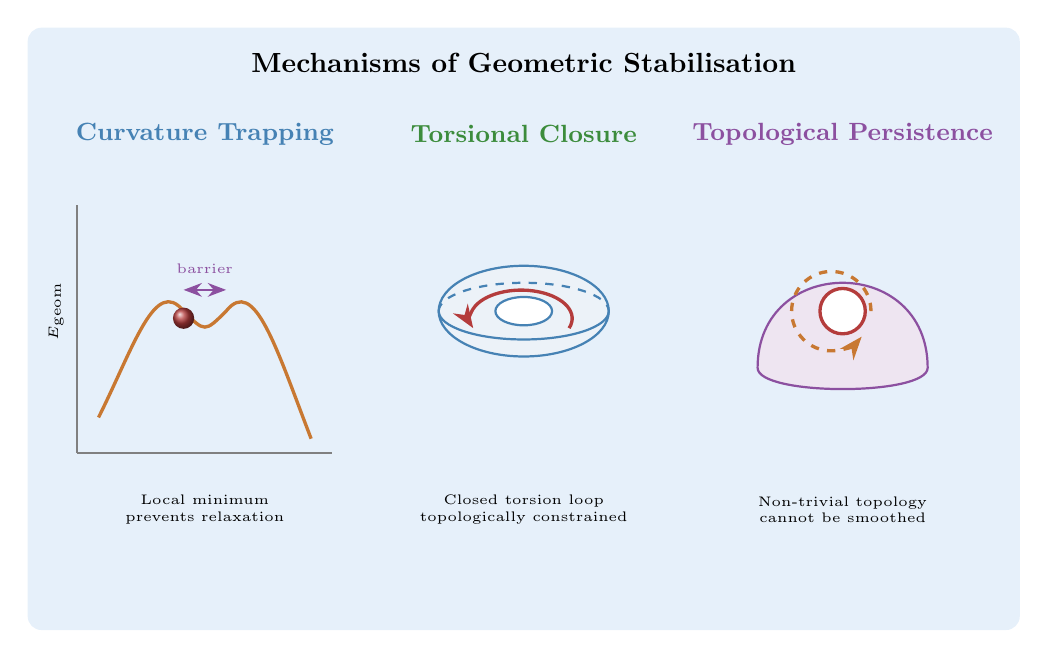
\begin{tikzpicture}[scale=0.9]
    % Background
    \fill[substrate, rounded corners=5pt] (-7,-4) rectangle (7,4.5);

    % Title
    \node[font=\bfseries] at (0,4) {Mechanisms of Geometric Stabilisation};

    % === Panel 1: Curvature Trapping ===
    \begin{scope}[shift={(-4.5,0.5)}]
        \node[font=\small\bfseries, curvature] at (0,2.5) {Curvature Trapping};

        % Energy landscape
        \draw[thick, gray] (-1.8,-2) -- (-1.8,1.5);
        \draw[thick, gray] (-1.8,-2) -- (1.8,-2);
        \node[font=\tiny, rotate=90] at (-2.1,0) {$E_{\text{geom}}$};

        % Double well potential
        \draw[very thick, energy] (-1.5,-1.5)
            .. controls (-1,-0.5) and (-0.7,0.5) .. (-0.3,0)
            .. controls (0,-0.3) and (0,-0.3) .. (0.3,0)
            .. controls (0.7,0.5) and (1,-0.5) .. (1.5,-1.8);

        % Ball in local minimum
        \shade[ball color=matter] (-0.3,-0.1) circle (0.15);

        % Barrier annotation
        \draw[{Stealth}-{Stealth}, thick, stable] (-0.3,0.3) -- (0.3,0.3);
        \node[font=\tiny, stable] at (0,0.6) {barrier};

        \node[font=\tiny, align=center] at (0,-2.8) {Local minimum\\prevents relaxation};
    \end{scope}

    % === Panel 2: Torsional Closure ===
    \begin{scope}[shift={(0,0.5)}]
        \node[font=\small\bfseries, relaxation] at (0,2.5) {Torsional Closure};

        % Torus with torsion loop
        \begin{scope}[scale=0.8]
            % Outer torus outline
            \draw[thick, curvature, fill=curvature!10] (0,0) ellipse (1.5 and 0.8);
            \draw[thick, curvature] (-1.5,0) arc (180:360:1.5 and 0.5);
            \draw[thick, curvature, dashed] (-1.5,0) arc (180:0:1.5 and 0.5);

            % Inner hole
            \fill[white] (0,0) ellipse (0.5 and 0.25);
            \draw[thick, curvature] (0,0) ellipse (0.5 and 0.25);

            % Torsion loop (highlighted)
            \draw[very thick, matter, -{Stealth}] (0.8,-0.3) arc (-20:200:0.9 and 0.5);
        \end{scope}

        \node[font=\tiny, align=center] at (0,-2.8) {Closed torsion loop\\topologically constrained};
    \end{scope}

    % === Panel 3: Topological Persistence ===
    \begin{scope}[shift={(4.5,0.5)}]
        \node[font=\small\bfseries, stable] at (0,2.5) {Topological Persistence};

        % Punctured surface
        \begin{scope}[scale=0.8]
            \draw[thick, stable, fill=stable!15]
                (-1.5,-1) .. controls (-1.5,1) and (1.5,1) .. (1.5,-1)
                .. controls (1.5,-1.5) and (-1.5,-1.5) .. (-1.5,-1);

            % Puncture/handle
            \draw[very thick, matter, fill=white] (0,0) circle (0.4);

            % Non-contractible loop
            \draw[very thick, energy, -{Stealth}, dashed]
                (0.5,0) arc (0:320:0.7);
        \end{scope}

        \node[font=\tiny, align=center] at (0,-2.8) {Non-trivial topology\\cannot be smoothed};
    \end{scope}
\end{tikzpicture}
\caption{Three stabilisation mechanisms. \textbf{Left:} Curvature trapping in a local energy minimum. \textbf{Centre:} Torsional closure forming a constrained loop. \textbf{Right:} Topological persistence from non-contractible structure.}
\label{fig:mechanisms}
\end{figure}

\subsection{The Definition Stated}
\label{subsec:definition-stated}

Matter is any geometric configuration satisfying the stabilisation conditions and persisting under relaxation dynamics due to curvature trapping, torsional closure, topological persistence, or their combination.

This definition is operational: given a geometric substrate and relaxation dynamics, ``matter'' denotes configurations meeting the stated criteria. The definition admits identification of matter configurations from geometric data alone.

\medskip
\noindent\textit{Takeaway:} Matter is defined as stabilised geometry---configurations that resist the relaxation from which gravity emerges.

% ============================================
% SECTION 5: MASS, INERTIA, COUPLING
% ============================================
\section{Mass, Inertia, and Gravitational Coupling}
\label{sec:mass-inertia}

If matter is stabilised geometry, then its gravitational properties must follow from geometric characteristics.

\subsection{Mass as Geometric Stiffness}
\label{subsec:mass}

The mass of a matter configuration can be related to the stiffness of the geometric energy functional at the stabilised configuration. Let $q$ denote a collective displacement coordinate parameterising deviations from equilibrium. The energy change under small displacement is:
\begin{equation}
\label{eq:energy-expansion}
\Delta \Egeom \approx \frac{1}{2} k \, q^2, \qquad
k := \left.\frac{\partial^2 \Egeom}{\partial q^2}\right|_{q=0}
\end{equation}

The parameter $k$ measures geometric stiffness: resistance to displacement from equilibrium. An effective inertial scale $\meff$ is expected to be a monotone function of this stiffness once a kinetic term for collective deformations is specified. For an effective Lagrangian $L = \frac{1}{2}\meff \dot{q}^2 - \frac{1}{2}k q^2$, the response timescale satisfies $\tau \sim \sqrt{\meff/k}$.

Configurations with larger stiffness $k$ are expected to exhibit greater inertial resistance, all else being equal; those with smaller $k$ respond more readily to perturbation. The precise relationship between $k$ and $\meff$ depends on the kinetic structure of the effective dynamics, which is not derived here.

\begin{figure}[H]
\centering
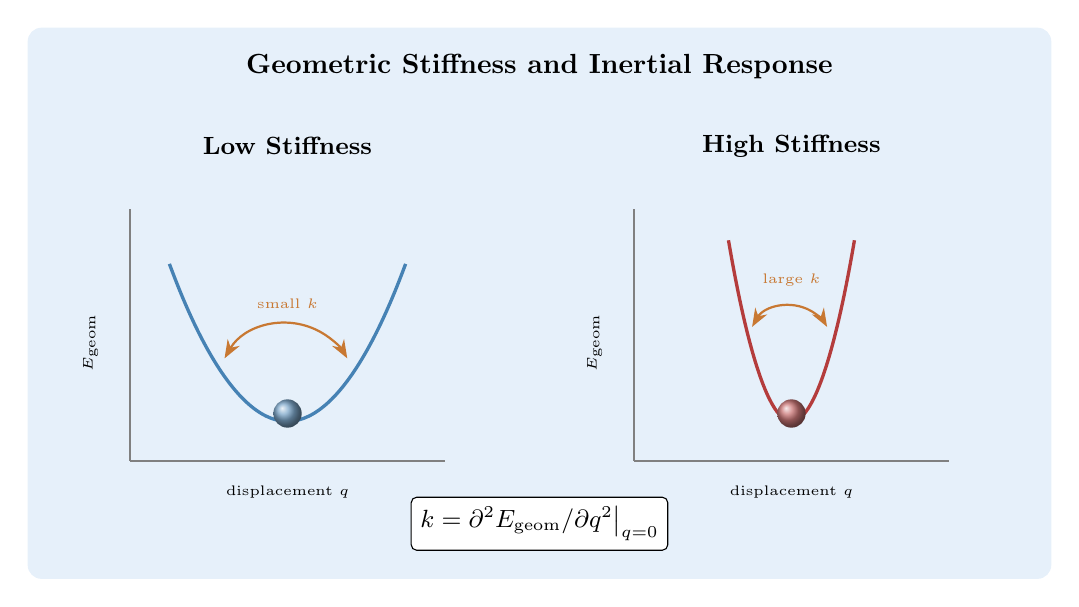
\begin{tikzpicture}[scale=1.0]
    % Background
    \fill[substrate, rounded corners=5pt] (-6.5,-3.5) rectangle (6.5,3.5);

    % Title
    \node[font=\bfseries] at (0,3) {Geometric Stiffness and Inertial Response};

    % Left panel: Low stiffness (shallow well)
    \begin{scope}[shift={(-3.2,0)}]
        \node[font=\small\bfseries] at (0,2) {Low Stiffness};

        % Axes
        \draw[thick, gray] (-2,-2) -- (-2,1.2);
        \draw[thick, gray] (-2,-2) -- (2,-2);
        \node[font=\tiny] at (0,-2.4) {displacement $q$};
        \node[font=\tiny, rotate=90] at (-2.5,-0.5) {$E_{\text{geom}}$};

        % Shallow parabola
        \draw[very thick, curvature] (-1.5,0.5) parabola bend (0,-1.5) (1.5,0.5);

        % Ball
        \shade[ball color=curvature!70] (0,-1.4) circle (0.18);

        % Curvature indicator
        \draw[{Stealth}-{Stealth}, thick, energy] (-0.8,-0.7) arc (150:30:0.9);
        \node[font=\tiny, energy] at (0,0) {small $k$};
    \end{scope}

    % Right panel: High stiffness (steep well)
    \begin{scope}[shift={(3.2,0)}]
        \node[font=\small\bfseries] at (0,2) {High Stiffness};

        % Axes
        \draw[thick, gray] (-2,-2) -- (-2,1.2);
        \draw[thick, gray] (-2,-2) -- (2,-2);
        \node[font=\tiny] at (0,-2.4) {displacement $q$};
        \node[font=\tiny, rotate=90] at (-2.5,-0.5) {$E_{\text{geom}}$};

        % Steep parabola
        \draw[very thick, matter] (-0.8,0.8) parabola bend (0,-1.5) (0.8,0.8);

        % Ball
        \shade[ball color=matter!70] (0,-1.4) circle (0.18);

        % Curvature indicator
        \draw[{Stealth}-{Stealth}, thick, energy] (-0.5,-0.3) arc (150:30:0.55);
        \node[font=\tiny, energy] at (0,0.3) {large $k$};
    \end{scope}

    % Equation
    \node[font=\small, draw, fill=white, rounded corners=2pt] at (0,-2.8)
        {$k = \partial^2 E_{\text{geom}}/\partial q^2 \big|_{q=0}$};
\end{tikzpicture}
\caption{Geometric stiffness. Shallow energy well (left) corresponds to low stiffness and weaker inertial response; steep well (right) corresponds to high stiffness and greater inertial resistance.}
\label{fig:mass-stiffness}
\end{figure}

\subsection{Inertia as Geometric Persistence}
\label{subsec:inertia}

Inertia is the tendency of a body to maintain its state of motion. For stabilised geometry, this persistence is automatic: stabilisation conditions ensure the configuration does not spontaneously change. External influence is required to alter the state.

When external perturbation is applied, the stabilised configuration adjusts its position within the substrate while maintaining internal structure. The rate of adjustment depends on stiffness: configurations with larger $k$ (higher effective mass) adjust more slowly.

This provides a geometric account of Newton's first law: stabilised configurations persist in their state unless acted upon by geometric perturbations.

\subsection{Gravitational Coupling}
\label{subsec:coupling}

The equivalence principle asserts that gravitational mass equals inertial mass. In the present framework, both derive from the same geometric characteristic: the stiffness of the energy functional at the stabilised configuration. No separate postulate is required to account for their common geometric origin.

Moreover, stabilised configurations curve the surrounding substrate because they \emph{are} configurations of the substrate. A localised region of non-trivial curvature affects adjacent regions through the same relaxation dynamics from which gravity emerges. The influence propagates outward as curvature redistributes.

This propagation manifests at macroscopic scales as the gravitational field. The matter configuration does not ``source'' curvature as an external agent; it \emph{is} a curvature configuration continuous with the substrate.

\begin{figure}[H]
\centering
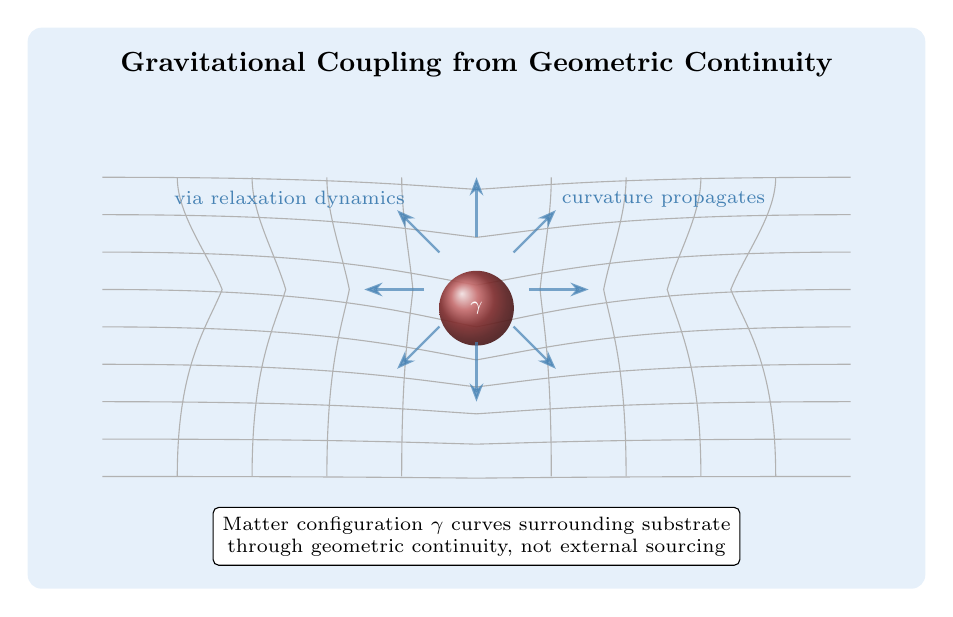
\begin{tikzpicture}[scale=0.95]
    % Background
    \fill[substrate, rounded corners=5pt] (-6,-4) rectangle (6,3.5);

    % Title
    \node[font=\bfseries] at (0,3) {Gravitational Coupling from Geometric Continuity};

    % Grid representing substrate (deformed)
    \begin{scope}
        % Horizontal lines (curved near center)
        \foreach \y in {-2.5,-2,-1.5,-1,-0.5,0,0.5,1,1.5} {
            \draw[thin, gray!60]
                (-5,\y) .. controls (-2,\y) and (-1,{\y-0.3*exp(-\y*\y/2)}) ..
                (0,{\y-0.5*exp(-\y*\y/2)})
                .. controls (1,{\y-0.3*exp(-\y*\y/2)}) and (2,\y) .. (5,\y);
        }

        % Vertical lines (curved near center)
        \foreach \x in {-4,-3,-2,-1,1,2,3,4} {
            \draw[thin, gray!60]
                (\x,-2.5) .. controls (\x,-1) and ({\x*0.9},-0.5) ..
                ({\x*0.85},0)
                .. controls ({\x*0.9},0.5) and (\x,1) .. (\x,1.5);
        }
    \end{scope}

    % Central matter configuration
    \shade[ball color=matter, opacity=0.9] (0,-0.25) circle (0.5);
    \node[font=\scriptsize, white] at (0,-0.25) {$\gamma$};

    % Curvature propagation arrows
    \foreach \angle in {0,45,90,135,180,225,270,315} {
        \draw[-{Stealth}, thick, curvature, opacity=0.7]
            ({\angle}:0.7) -- ({\angle}:1.5);
    }

    % Labels
    \node[font=\scriptsize, curvature] at (2.5,1.2) {curvature propagates};
    \node[font=\scriptsize, curvature] at (-2.5,1.2) {via relaxation dynamics};

    % Caption box
    \node[font=\scriptsize, align=center, draw, fill=white, rounded corners=2pt] at (0,-3.3)
        {Matter configuration $\gamma$ curves surrounding substrate\\
        through geometric continuity, not external sourcing};
\end{tikzpicture}
\caption{Gravitational coupling as geometric continuity. A stabilised configuration $\gamma$ influences surrounding geometry through the same relaxation dynamics that produce gravity.}
\label{fig:coupling}
\end{figure}

\medskip
\noindent\textit{Takeaway:} Geometric stiffness underlies both inertial and gravitational response; the equivalence principle follows without additional postulates.

% ============================================
% SECTION 6: SCALE TRANSITION
% ============================================
\section{Scale Transition and Emergence of Discreteness}
\label{sec:discreteness}

The stabilisation conditions restrict the space of allowed configurations, with implications for the transition between continuous and discrete descriptions.

\subsection{Stabilisation Implies Selection}
\label{subsec:selection}

Not every geometric configuration is stabilised. The conditions $\delta \Egeom = 0$ and $\delta^2 \Egeom > 0$ typically select a discrete or countable set (up to symmetries) from the continuous space of possibilities. Allowed configurations correspond to local minima; those not satisfying stabilisation conditions relax away.

This selection is analogous to quantisation of normal modes in bounded systems: continuous parameters are reduced to discrete values by boundary or stability conditions.

\subsection{Topological Quantisation}
\label{subsec:topological}

Where stabilisation involves topological persistence, the relevant invariants are inherently discrete. Topological charges, winding numbers, and similar quantities take integer values. If matter configurations are characterised by such invariants, the spectrum of allowed configurations is automatically discrete.

For configurations involving closed geometric structures, we write a representative schematic closure condition of the form:
\begin{equation}
\label{eq:topological-quantisation}
\oint_C \Gamma = 2\pi n
\end{equation}
where $\Gamma$ represents a geometric quantity integrated around a closed curve $C$, and $n$ is an integer. Such conditions arise generically from continuity requirements on multi-valued geometric objects.

\subsection{Mode Structure}
\label{subsec:modes}

The stabilisation conditions define a spectrum of allowed configurations indexed by discrete labels. Let $\gamma_n$ denote the configuration corresponding to mode index $n$. Each $\gamma_n$ has an associated energy $E_n = \Egeom[\gamma_n]$ and characteristic geometry.

The discreteness of this spectrum is the geometric precursor to quantum behaviour in the present framework. Transitions between configurations involve discontinuous changes in topological or stability characteristics, with corresponding discrete energy differences.

\begin{figure}[H]
\centering
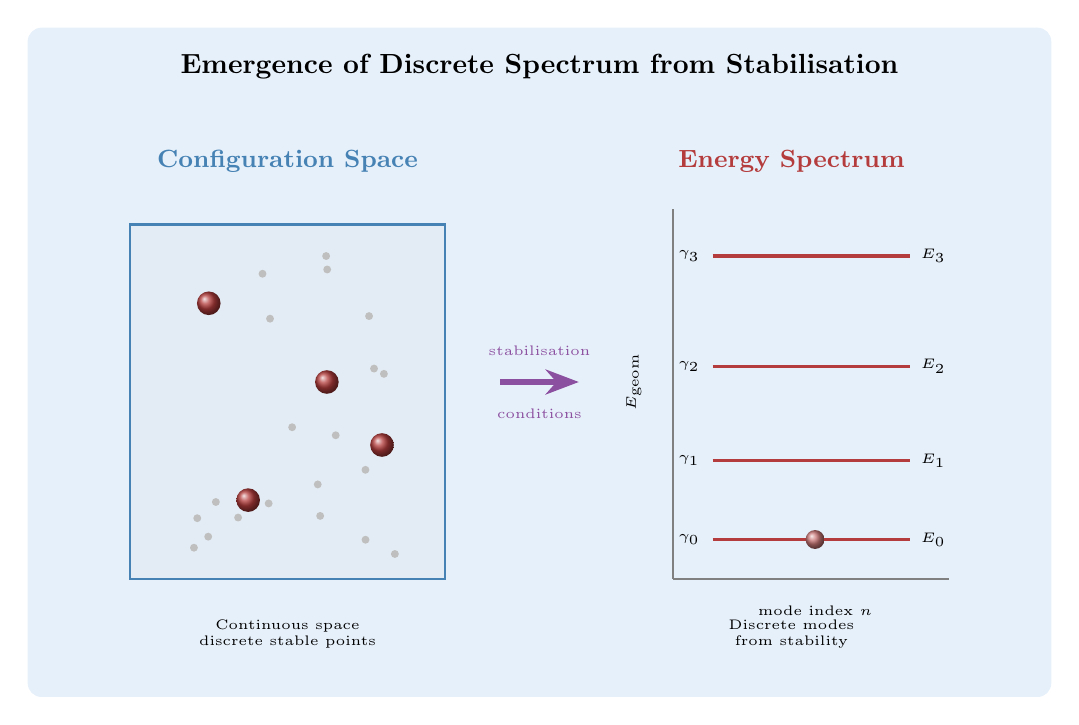
\begin{tikzpicture}[scale=1.0]
    % Background
    \fill[substrate, rounded corners=5pt] (-6.5,-4) rectangle (6.5,4.5);

    % Title
    \node[font=\bfseries] at (0,4) {Emergence of Discrete Spectrum from Stabilisation};

    % Left panel: Configuration space
    \begin{scope}[shift={(-3.2,0)}]
        \node[font=\small\bfseries, curvature] at (0,2.8) {Configuration Space};

        % Continuous space (shaded region)
        \fill[curvature!15] (-2,-2.5) rectangle (2,2);
        \draw[thick, curvature] (-2,-2.5) rectangle (2,2);

        % Random points (unstable configurations) - using rnd [0,1] for proper bounds
        \foreach \i in {1,...,20} {
            \pgfmathsetmacro{\x}{-1.7+3.4*rnd}
            \pgfmathsetmacro{\y}{-2.2+3.9*rnd}
            \fill[gray!50] (\x,\y) circle (0.05);
        }

        % Stable configurations (highlighted)
        \shade[ball color=matter] (-1,1) circle (0.15);
        \shade[ball color=matter] (0.5,0) circle (0.15);
        \shade[ball color=matter] (-0.5,-1.5) circle (0.15);
        \shade[ball color=matter] (1.2,-0.8) circle (0.15);

        \node[font=\tiny, align=center] at (0,-3.2) {Continuous space\\discrete stable points};
    \end{scope}

    % Arrow
    \draw[-{Stealth}, very thick, stable, line width=2pt] (-0.5,0) -- (0.5,0);
    \node[font=\tiny, stable] at (0,0.4) {stabilisation};
    \node[font=\tiny, stable] at (0,-0.4) {conditions};

    % Right panel: Energy spectrum
    \begin{scope}[shift={(3.2,0)}]
        \node[font=\small\bfseries, matter] at (0,2.8) {Energy Spectrum};

        % Energy axis
        \draw[thick, gray] (-1.5,-2.5) -- (-1.5,2.2);
        \draw[thick, gray] (-1.5,-2.5) -- (2,-2.5);
        \node[font=\tiny, rotate=90] at (-2,0) {$E_{\text{geom}}$};
        \node[font=\tiny] at (0.3,-2.9) {mode index $n$};

        % Discrete energy levels
        \draw[very thick, matter] (-1,-2) -- (1.5,-2);
        \node[font=\tiny] at (1.8,-2) {$E_0$};
        \node[font=\tiny] at (-1.3,-2) {$\gamma_0$};

        \draw[very thick, matter] (-1,-1) -- (1.5,-1);
        \node[font=\tiny] at (1.8,-1) {$E_1$};
        \node[font=\tiny] at (-1.3,-1) {$\gamma_1$};

        \draw[very thick, matter] (-1,0.2) -- (1.5,0.2);
        \node[font=\tiny] at (1.8,0.2) {$E_2$};
        \node[font=\tiny] at (-1.3,0.2) {$\gamma_2$};

        \draw[very thick, matter] (-1,1.6) -- (1.5,1.6);
        \node[font=\tiny] at (1.8,1.6) {$E_3$};
        \node[font=\tiny] at (-1.3,1.6) {$\gamma_3$};

        % Balls on levels
        \shade[ball color=matter!70] (0.3,-2) circle (0.12);

        \node[font=\tiny, align=center] at (0,-3.2) {Discrete modes\\from stability};
    \end{scope}
\end{tikzpicture}
\caption{Emergence of discreteness. Left: Continuous configuration space with stable configurations (red) satisfying $\delta E = 0$, $\delta^2 E > 0$. Right: Stable configurations form a discrete spectrum of modes $\gamma_n$ with energies $E_n$.}
\label{fig:discreteness}
\end{figure}

\subsection{Limitation}
\label{subsec:limitation}

The foregoing describes the origin of discreteness but does not constitute a derivation of quantum dynamics. Superpositions, interference, and probabilistic aspects require additional structure beyond stabilisation conditions. These developments are deferred to subsequent work.

\medskip
\noindent\textit{Takeaway:} Discreteness emerges from stabilisation constraints; full quantum dynamics remain to be derived.

% ============================================
% SECTION 7: SCOPE AND NON-CLAIMS
% ============================================
\section{Scope and Non-Claims}
\label{sec:scope}

To prevent misunderstanding, we state explicitly what this paper does \textbf{not} claim.

\begin{enumerate}[leftmargin=2em, label=(\roman*)]
    \item \textbf{This paper does not replace quantum field theory.} The Standard Model remains the empirically successful framework for describing matter and its interactions. The relationship between geometric stabilisation and quantum field theory is not established here.

    \item \textbf{This paper does not derive particle spectra.} The observed spectrum of elementary particles---masses, charges, quantum numbers---is not derived. The framework suggests such a spectrum might emerge from stabilisation conditions, but no derivation is provided.

    \item \textbf{This paper does not derive fermion dynamics.} Spin-1/2 particles, spinor fields, and the Dirac equation are not addressed.

    \item \textbf{This paper does not claim unification.} Unifying gravity with other fundamental forces remains an open problem. The claim here is limited: matter can be defined as stabilised geometry, with mass and inertia following from geometric characteristics.

    \item \textbf{This paper does not introduce new fundamental entities.} No new particles, fields, or forces are postulated. All physical content derives from the geometric substrate and its dynamics.

    \item \textbf{This paper does not rederive gravity.} The results of BP3 are assumed. Gravity enters as a foundational constraint, not a derived consequence.
\end{enumerate}

The contribution is definitional and conceptual: clarifying matter's ontological status within emergent gravity. Whether this framework can be developed into a complete theory of matter remains open.

% ============================================
% SECTION 8: DISCUSSION AND OUTLOOK
% ============================================
\section{Discussion and Outlook}
\label{sec:discussion}

Within an emergent gravity framework, ontological consistency requires matter to be understood as stabilised geometry. This is not an additional hypothesis but a logical implication of treating gravity as emergent from a single geometric substrate. The definition of matter as configurations resisting relaxation provides a natural account of mass, inertia, and gravitational coupling.

The principal limitation is generality. We have described what matter must be, not what configurations exist. A discrete spectrum of stabilised configurations should arise from the interplay of curvature dynamics, torsional closure, and topological persistence. But specific configurations depend on details of the energy functional and the substrate at small scales.

The immediate task for subsequent work (BP4) is to characterise the stabilisation modes:

\begin{enumerate}[leftmargin=2em]
    \item Specification of the geometric energy functional, including curvature, torsion, non-metricity, and their derivatives.

    \item Analysis of the functional's critical points to identify stabilised configurations.

    \item Classification of configurations by topological invariants and stability type.

    \item Derivation of effective dynamics governing transitions between configurations.
\end{enumerate}

The final item is essential for contact with quantum theory. If correct, the effective dynamics of stabilised configurations should reproduce---or be compatible with---observed quantum dynamics. This is a strong requirement and a critical test.

\begin{figure}[H]
\centering
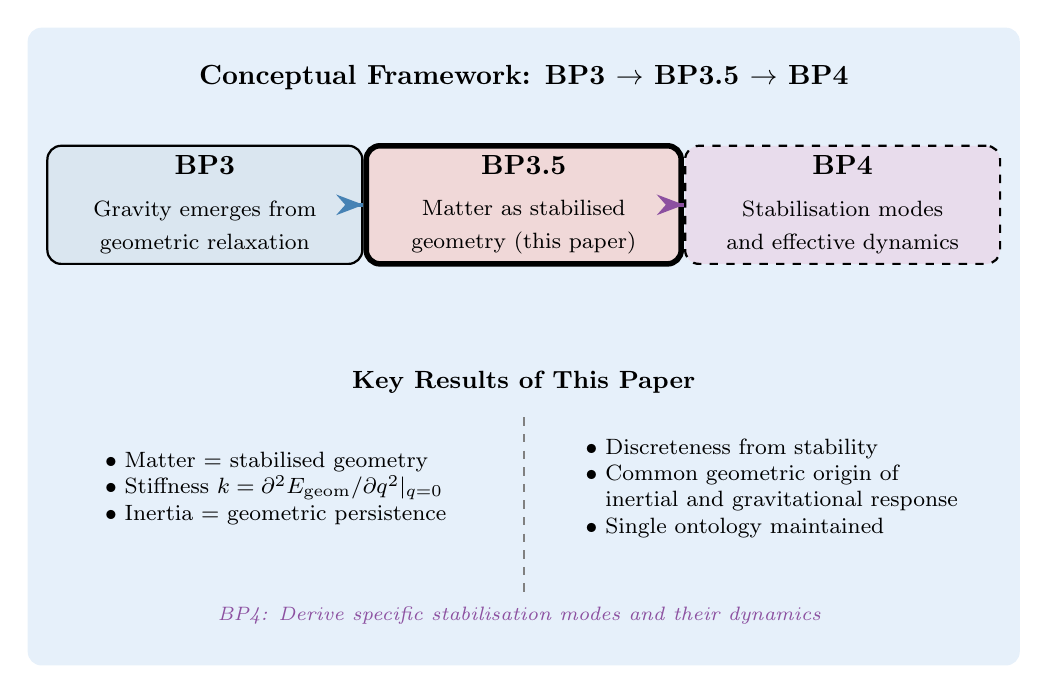
\begin{tikzpicture}[
    box/.style={draw, thick, rounded corners=5pt, minimum width=4cm, minimum height=1.5cm, align=center, fill=white},
    arrow/.style={-{Stealth}, thick, line width=1.5pt},
    scale=0.9
]
    % Background
    \fill[substrate, rounded corners=5pt] (-7,-5) rectangle (7,4);

    % Title
    \node[font=\bfseries] at (0,3.3) {Conceptual Framework: BP3 $\to$ BP3.5 $\to$ BP4};

    % BP3 box
    \node[box, fill=curvature!20] (bp3) at (-4.5,1.5) {
        \textbf{BP3}\\[0.3em]
        \footnotesize Gravity emerges from\\
        \footnotesize geometric relaxation
    };

    % BP3.5 box (this paper)
    \node[box, fill=matter!20, line width=2pt] (bp35) at (0,1.5) {
        \textbf{BP3.5}\\[0.3em]
        \footnotesize Matter as stabilised\\
        \footnotesize geometry (this paper)
    };

    % BP4 box
    \node[box, fill=stable!20, dashed] (bp4) at (4.5,1.5) {
        \textbf{BP4}\\[0.3em]
        \footnotesize Stabilisation modes\\
        \footnotesize and effective dynamics
    };

    % Arrows
    \draw[arrow, curvature] (bp3) -- (bp35);
    \draw[arrow, stable] (bp35) -- (bp4);

    % Lower panel: Key results
    \node[font=\small\bfseries] at (0,-1) {Key Results of This Paper};

    \node[font=\footnotesize, align=left] at (-3.5,-2.5) {
        $\bullet$ Matter $=$ stabilised geometry\\
        $\bullet$ Stiffness $k = \partial^2 E_{\text{geom}}/\partial q^2|_{q=0}$\\
        $\bullet$ Inertia $=$ geometric persistence
    };

    \node[font=\footnotesize, align=left] at (3.5,-2.5) {
        $\bullet$ Discreteness from stability\\
        $\bullet$ Common geometric origin of\\
        \hspace{0.5em} inertial and gravitational response\\
        $\bullet$ Single ontology maintained
    };

    % Divider
    \draw[thick, gray, dashed] (0,-1.5) -- (0,-4);

    % Future work note
    \node[font=\scriptsize, stable, align=center] at (0,-4.3) {
        \textit{BP4: Derive specific stabilisation modes and their dynamics}
    };
\end{tikzpicture}
\caption{Progression of the Bridge Papers series. BP3 established emergent gravity. BP3.5 (this paper) defines matter as stabilised geometry. BP4 will characterise specific modes and derive effective dynamics.}
\label{fig:framework}
\end{figure}

We conclude with a summary. If gravity emerges from geometric relaxation, matter cannot be ontologically separate from geometry. Matter must consist of geometric configurations that resist relaxation. This identification is required by the internal logic of emergent gravity. The consequences---geometric stiffness underlying inertial response, geometric persistence, discreteness from stabilisation---follow as necessary implications. Whether these accord with observation, and whether the framework yields a predictive theory of matter, remains to be determined.

% ============================================
% ACKNOWLEDGMENTS
% ============================================
\section*{Acknowledgments}

This work builds on the foundational analysis of BP3. No external funding supported this research.

% ============================================
% REFERENCES
% ============================================
\begin{thebibliography}{99}

\bibitem{BP3}
L.~Smart, ``On the Emergence of Gravitational Dynamics from Geometric Relaxation,'' BP3, Vibrational Field Dynamics Institute, 2025.

\bibitem{future}
Further references to be added upon integration with existing literature on emergent gravity, geometric mechanics, and topological aspects of field theory.

\end{thebibliography}

\end{document}
